
{\bf \Huge Research Plan} \\[0.5cm]

  My research is divided into two phases, a research project in the fall and master thesis in the following spring. This research plan will cover both phases.

  \section*{Purpose}

  %Describe the reason for doing the research, the topic of interest, why it is important or useful to study this, the specific research question( s) asked and the objectives set. Research without a purpose is unlikely to be good research."

  In todays society, people tends to spend a lot of time on their mobile devices. Mobile devices are not just a communication tool, but also an important tool for everyday tasks like doing our work, reading mail, pay our bills, and keeping up with our social life. Our whole life is contained in one device. When such a small device is so important it makes it vulnerable in terms of security.

  Passwords are human-chosen secrets that are connected to you as a person. When the password is created you might create a password that is an association to something you know or recognize; passwords are more than just words and numbers. Because of the shortcomings of text-based passwords \cite{UnixPasswords}, there is an increased interest in graphical passwords. The interest in graphical passwords started with the assumption that pictures are easier to remember and more secure than words and numbers \cite{DeAngeli}. Google's Android platform released the functionality for the Android Unlock Pattern in 2008, that is a security mechanism for locking Android smartphones. Since its release, there have been a lot of discussion regarding its security, but little scientific research on the Android Unlock Pattern. The problem is not just the theoretical password space, but the password space in practice. 

  The motivation for this thesis started by observing the shortcomings of graphical passwords. Password reuse is one of the known password habits among users because of the human limitation in remembering text-based passwords. Some users also make simple or semantic passwords that are easier to remember, making their passwords vulnerable to attacks. Graphical passwords look like a promising alternative to text-based passwords, as it aids users in remembering and create more complex passwords, offering increased usability and higher security. As mobile devices play an important role in our everyday life, this makes it an interesting target device. Security on mobile devices have changed during the past years. Historically, locking mechanisms were a solution solely to prevent accidental use, while current mobile phones require protection in order to secure the potentially vast amount of private data that we keep on them.

  In 2013 a research group conducted the first large-scale user study on the Android Unlock Patterns \cite{Uellenbeck}. The outcome of the research was an analysis of 2900 collected Android Unlock Patterns. They found a lot of bias in the pattern making process claiming that the scheme is less secure than its theoretical password space. 

  My research aims to take the analysis of people's choice in Android Unlock Patterns a step further by including the human properties that may impact the user choice in graphical passwords. The study adds to the body of knowledge by testing the hypothesis that human properties affects user's choice of graphical passwords. It is also desired to look into further improvements of the scheme. 

  {\bf $RQ1$: What is the status of current research on graphical passwords?}

  {\bf $RQ2$: What human properties may affect our choice of graphical passwords on mobile devices?}

  {\bf $RQ3$: How is users choice of patterns based on human properties affecting the security of the Android Unlock Pattern?}

  {\bf $RQ3.1$: If any security risks is observed, how could the Android Unlock Pattern scheme be improved in order to reduce the security risks?} 
  
  \section*{Products}

  The main product of this research is to test a hypothesis in mobile security. The hypothesis states that there is a connection between users' choice in graphical passwords based on human properties like physical conditions and demographics. Towards reaching this goal, there are other sub-products of the research process. The literature review and the research design is two sub-products delivered in the project thesis. In my master thesis, a data collection and quantitative data analysis is conducted. The data itself is a valuable product, and alongside with the analysis, it can provide answers to the hypothesis.

  Research on passwords is not easy to conduct because of the nature of passwords. Passwords should not be shared. Research on text-based passwords is often based on leaked password on the web. When analyzing Android Unlock Patterns, there is no such data source available. This research design can provide insight into a new way of solving the problem of collecting user chosen passwords on mobile devices. The research design provides a detailed description of the strategy chosen to collect Android Unlock Patterns from users through a questionnaire over the Internet. This can provide knowledge for future research on graphical passwords on mobile devices. 
  
  \section*{Process}

  \begin{wrapfigure}{l}{0.53\textwidth}
     \vspace{-20pt}
     \begin{center}
        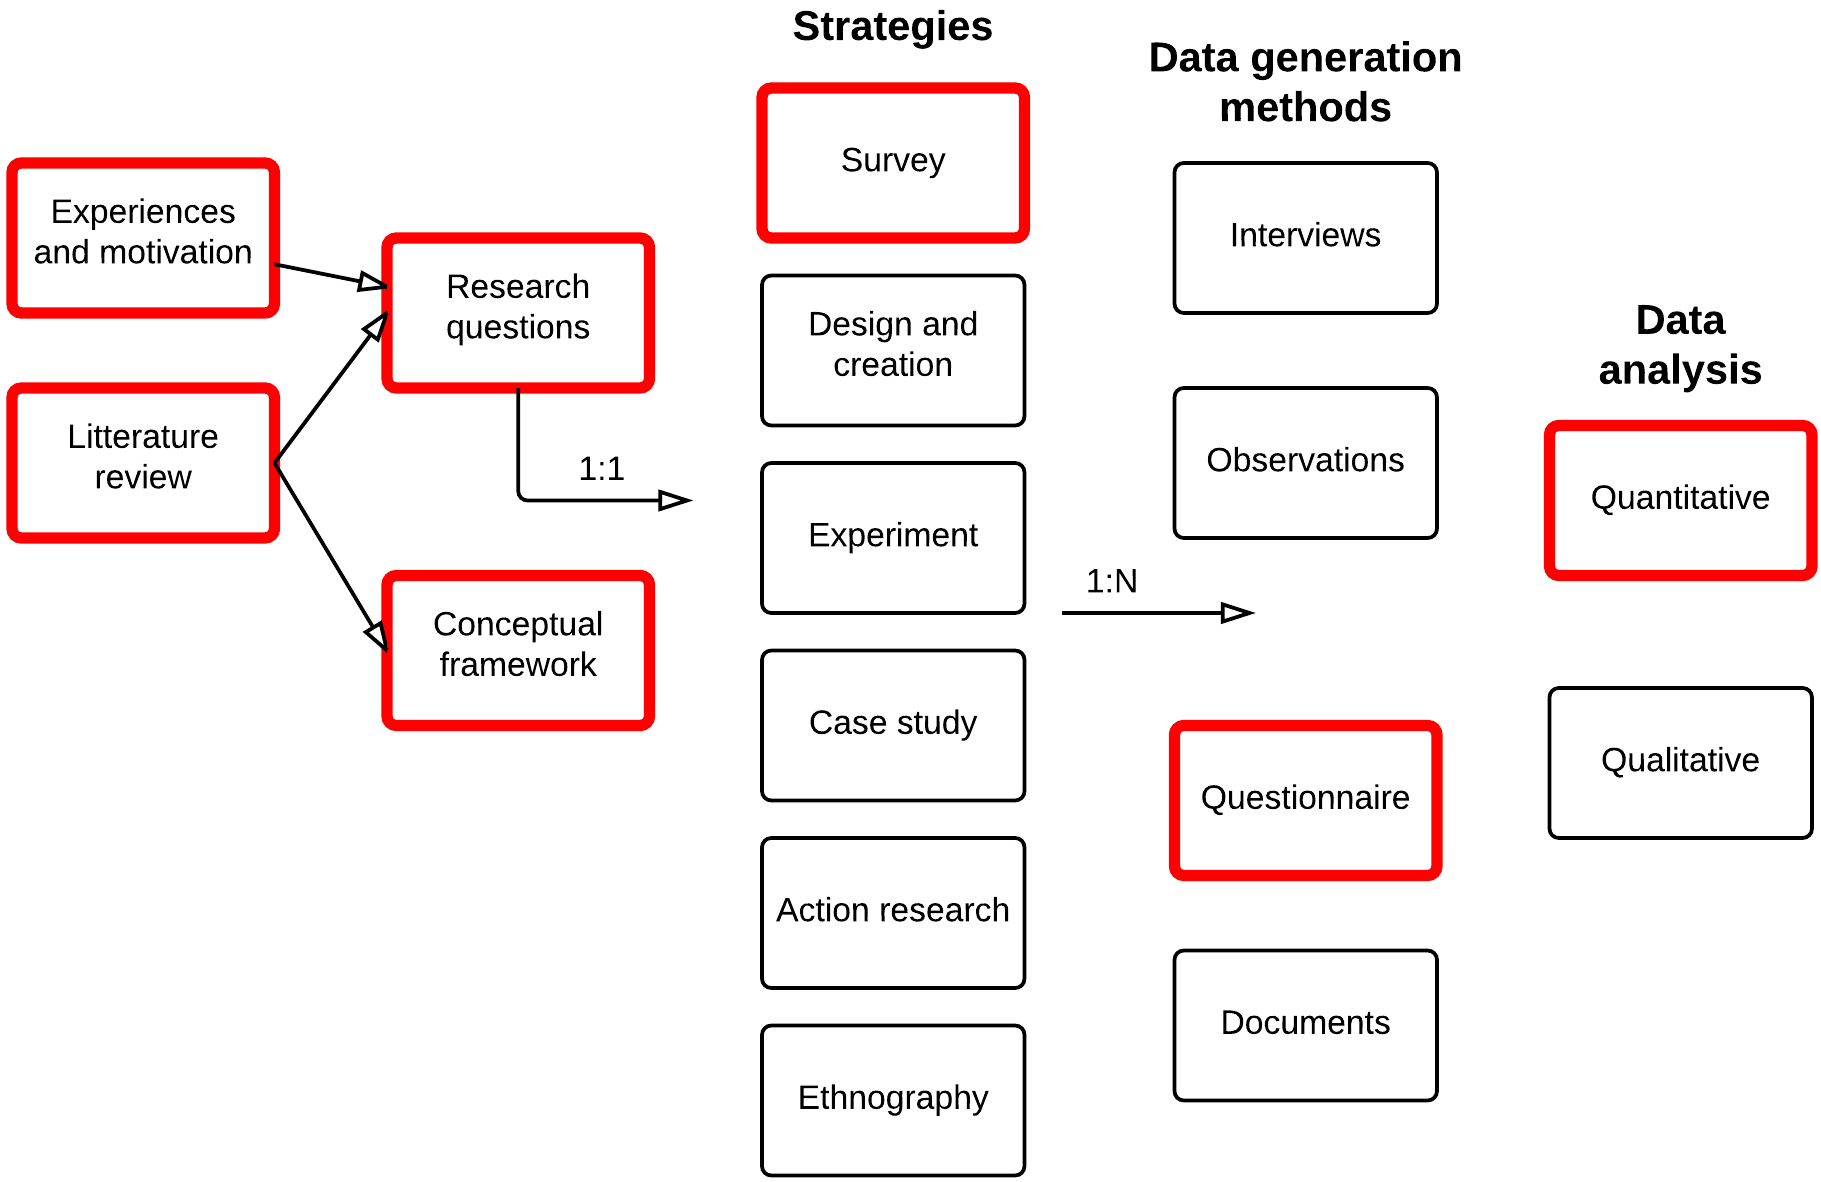
\includegraphics[scale=0.13]{ResearchProcess.png}
     \end{center}
     \vspace{-5pt}
     \caption{Research Process \cite{empiriske}}
   \end{wrapfigure}

  This research spurred by the experience and motivation that graphical passwords are an interesting form of authentication, supporting users to remember more complex passwords that should provide better security. To find the research questions, I started with a literature review, providing a conceptual framework for the thesis. From the literature review, I found that there is a lack of research on human choices of graphical passwords based on human properties. Beside the literature review, the research project also includes a research design for my master thesis. In order to find out if there is possible to see a pattern between users choice in passwords and human properties, a survey is planned along with a questionnaire for the data collection. The research requires a large sample of data for finding patterns in users' choice of Android Unlock Patterns, as well as diversity in the data in terms of demographics. With today's technology it is possible to distribute the questionnaire over the Internet. A questionnaire also provides a standardized format of the data that can be helpful for the analysis. The selected research strategy and data generation method will provide quantitative data for the analysis.

  \section*{Participants}

  As a researcher, I am included as a participant. My work is to plan and conduct the research. 

  The research is supervised by Lillian Røstad and Per Thorsheim. Lillian is my main supervisor and is contributing with her experience with research in computer science and security. Per has the role as my co-supervisor and is an external participant outside of the academic field. He is contributing in this research because of his personal interest in passwords and security, as well as providing a network of contacts within the field of information security. Both have the right to the results form this research.

  In this research, there is not a narrow target population. The aim is to collect data world wide: Everyone with a smartphone is considered a part of the target population. All the volunteered respondents are considered participants in this research. Myself, as a researcher, have no personal contact with the respondents, but need to carefully handle the information from the respondents according to a legal and ethical perspective. It should not be able to track the information back to the respondents. All the data from the respondents are kept anonymous and will not be used outside of this research. Information concerning legal and ethical aspects of this research should be described in the questionnaire. 

  \section*{Paradigm}
  With a survey as the a chosen research strategy, this research seeks to find patterns that are assumed to exist. This is a way of thinking is closely related to the positivism paradigm. This research is based on empirical testing of a hypothesis, with a desire to confirm or refuse the assumptions made in the hypothesis.
  When conducting the research, my beliefs as a researcher are independent of my research and my research can be stated to be objective. It is conducted with minimal interaction with the participants and the research is based on facts, that is the the quantitative data collected. 

  \section*{Presentation}
  The presentation of the result from this research will be presented in two deliverable documents, project thesis and master thesis. The research will also be presented at the conference ``Passwords14''\cite{passwords} in December. The presentation will provide insightful feedback from researcher, as well as providing knowledge about the gap in the research on graphical passwords. 



  \section*{References}
  \renewcommand{\bibsection}{ }
  \bibliographystyle{plain}
  \bibliography{mybib}







  